% Runtime CPS safety policy verification proposal (USENIX-style).
\documentclass[letterpaper,twocolumn,10pt]{article}

\usepackage{usenix}
\usepackage{amsmath,amssymb}
\usepackage{booktabs}
\usepackage{graphicx}
\usepackage{xspace}
\usepackage{tikz}
\usetikzlibrary{arrows.meta,positioning}

\newcommand{\SafetyIsland}{safety island\xspace}
\newcommand{\SafetyIslands}{safety islands\xspace}
\newcommand{\STL}{STL\xspace}
\newcommand{\FTTI}{FTTI\xspace}
\newcommand{\PrimaryCompute}{main CPU\xspace}

\begin{document}
\date{}

\title{\Large \bf Cache-Coherent Safety Islands for Low-Latency CPS Policy Monitoring}

\author{
{\rm Nazmus Shakib Sayom}\\
University of Utah
}

\maketitle
\thispagestyle{empty}

\begin{abstract}
Many safety-critical cyber-physical systems (CPS) include a \SafetyIsland: a small high-assurance microcontroller that supervises the \PrimaryCompute. This project proposes making cache-coherent shared memory the centerpiece of the safety-island monitoring architecture, so the controller can export intent with very low latency. We will study what coherence, ordering, and timing assumptions are needed so the \SafetyIsland can read consistent controller records, align them with independent actuation evidence, and evaluate temporal safety policies (e.g., \STL) within the fault-tolerant time interval (\FTTI).
\end{abstract}

\section{Motivation and Scope}
Functional safety standards require detecting and controlling faults fast enough to prevent hazards (within the fault-tolerant time interval, \FTTI)~\cite{ISO26262}. Many automotive systems-on-chip (SoCs) therefore include an isolated \SafetyIsland that can stay trustworthy under faults and supervise the rest of the system~\cite{ArmAutoSolutionsOverview,NVIDIADriveFSI,SiemensSI}. Today, these islands mostly run watchdogs, self-tests, and fault handling. This project asks what it would take, architecturally, for a \SafetyIsland to also run online checks of \emph{signal-level safety policies}.

We focus on actuation because it is where software intent meets hardware reality. Even when the controller code is correct, faults or timing perturbations in the actuation path can violate safety requirements before coarse supervision reacts. PWM-driven actuation is a representative case: the controller computes PWM parameters, but the downstream chain (register writes, peripherals, interconnect, gate driver, power stage) determines realized switching behavior.

Temporal logics such as Signal Temporal Logic (\STL) are a common way to write timing requirements over signals, and robust monitoring can provide a numeric ``margin'' that tolerates bounded noise~\cite{MalerNickovic2004,FainekosPappas2009,Deshmukh2017}. Cache-coherent shared memory is attractive for runtime verification under tight \FTTI budgets because it enables a low-latency, single-copy export path: the controller can write a record into shared memory and the \SafetyIsland can read it via ordinary loads.

The key architecture challenge is to make this coherent path \emph{both correct and time-bounded}. Correctness requires that multi-field controller records are read as consistent snapshots under weak ordering~\cite{Pulte2018SimplifyingARM}. Time-boundedness requires that the coherent export and monitor execution remain within worst-case latency budgets even under coherence and shared-interconnect contention~\cite{Hassan2017PredictableCoherence,Hassan2022IntegratingCOTSCoherence}.

\textbf{Hypothesis.} Cache-coherent shared memory is the right substrate for low-latency intent export to a \SafetyIsland monitor. We hypothesize that, with an explicit synchronization discipline for multi-field records and with predictability mechanisms for coherence contention, a microcontroller-class \SafetyIsland can perform robust temporal-policy monitoring (e.g., \STL) within the \FTTI.

\section{Related Work and Gap}
\subsection{Safety Islands in Automotive SoCs}
Modern automotive platforms already include safety islands. Arm Automotive Solutions platforms---including the Zena CSS subsystem~\cite{ArmZenaCSS} and the Kronos reference design~\cite{ArmAutoSolutionsOverview}---incorporate a safety island alongside application-class compute; Kronos further documents an explicit cross-domain messaging path (HIPC)~\cite{ArmHIPC}. NVIDIA's DriveOS documentation similarly describes a functional safety island with defined responsibilities and a controlled interface to the rest of the SoC~\cite{NVIDIADriveFSI}. A Siemens white paper makes the same case: keep safety-related control and safety/security/test data handling in a segregated subsystem aligned with ISO~26262 processes~\cite{SiemensSI}.

These sources establish \emph{isolation and communication mechanisms}, but they do not define the monitoring-oriented interface contract we need. In particular, they do not specify how to export controller intent as a coherent, consistently readable record (what constitutes a single ``step'' and how snapshots are formed) or how that record should align (in time) with independent actuation evidence. Our proposal asks whether a small, access-controlled cache-coherent shared-memory region can serve as the low-latency monitoring interface, and what correctness and predictability constraints that implies.

Arm's actuation-focused safety-island demo motivates actuation integrity supervision, but it still leaves open how to generalize to a sound interface contract across SoCs and communication fabrics~\cite{ArmActuationDemo}.

\subsection{Runtime Assurance and Runtime Verification}
Simplex-style runtime assurance uses a trusted supervisor to monitor an advanced controller and switch to a safe controller when needed~\cite{Sha1998SimplexACC,Sha2001UsingSimplicity}. Later work extends this pattern to resilient CPS upgrades and partially opaque (e.g., data-driven) controllers, while keeping the supervisor as the trusted base that decides when to fall back~\cite{Rutledge2018RSimplex,Yalcinkaya2023Ulgen,Desai2022BlackBoxSimplex}. This line of work clarifies \emph{what to do after detection}, but it typically assumes the monitor already receives a consistent view of the signals it checks.

Runtime verification provides the temporal monitoring foundations we need. Maler and Ni{\v c}kovi{\'c} define monitoring temporal properties over continuous signals~\cite{MalerNickovic2004}. Robust (quantitative) semantics assign a real-valued robustness degree, which is useful for tolerating bounded noise and turning ``how close to violation'' into a monitor output~\cite{FainekosPappas2009}. Robust online monitoring algorithms and tools (e.g., RTAMT) make \STL-style monitoring practical in streaming settings~\cite{Deshmukh2017,RTAMT2020}, and FPGA realizations show feasibility at high sampling rates~\cite{Dokhanchi2015FPGASTL}.

Two threads are especially relevant to a \SafetyIsland design. First, interface-aware \STL (IA-\STL) makes explicit that a monitor may only see signals through a component interface, and it defines semantics that account for this limitation (e.g., input/output roles and vacuity)~\cite{Ferrere2019IASTL}. Second, distributed \STL monitoring studies how monitoring changes when there is no single globally synchronized trace; for example, Momtaz et al.\ assume bounded clock drift in a partially synchronous model and use retiming plus SMT-based checks to decide satisfaction~\cite{Momtaz2023DistSTL}. Heterogeneous runtime verification explores placing monitors on different substrates (e.g., FPGA versus CPU) to meet tight deadlines~\cite{Gautham2020HeterogeneousRV}.

Taken together, these works provide strong semantics and monitoring algorithms, but they largely treat the input trace as already well-defined: signals are sampled, time-stamped, and delivered to the monitor in a way that corresponds to the intended physical timeline. A \SafetyIsland monitor must instead \emph{establish} that property across an isolation boundary.

\subsection{Cache-Coherent Sharing, Ordering, and Predictability}
Cache coherence provides a natural substrate for low-latency intent export: the \PrimaryCompute can write controller records into a shared region and the \SafetyIsland can read them without software-managed copying or cache maintenance, using standard coherent interfaces (e.g., Arm AMBA ACE/CHI-style protocols)~\cite{ArmAMBA4,ArmAMBA5}. However, coherence alone does not imply atomic multi-field snapshots. Weak ordering can still expose mixed old/new fields unless the interface contract includes explicit synchronization, which is especially relevant on Arm systems~\cite{Pulte2018SimplifyingARM}.

Coherent sharing also raises two additional challenges that are central to this project. First, the \PrimaryCompute and \SafetyIsland may not have identical memory-model behavior; recent work (MemGlue) shows that coherence protocols must be aware of memory-consistency requirements in heterogeneous systems to avoid mismatches~\cite{CleavelandTrippel2024MemGlue}. Compound memory models similarly motivate reasoning about the CPU--island interface as a composed contract, not a single monolithic ``system memory model''~\cite{Goens2023CompoundConsistency}.

Second, coherence can harm predictability: shared caches and coherence traffic introduce contention that can inflate worst-case latency. There is substantial real-time systems work on making coherence predictable (e.g., predictable coherence protocols and predictable integration of commodity coherent fabrics)~\cite{Hassan2017PredictableCoherence,Kaushik2021PredictableCoherence,Hassan2022IntegratingCOTSCoherence}. Mixed-criticality work also highlights the tension between strong isolation and efficient sharing on coherent multicore platforms~\cite{Chisholm2016TensionIsolationSharing}.

\textbf{Gap.} Safety-island platforms define isolation and basic communication paths~\cite{ArmHIPC,NVIDIADriveFSI}, cache coherence provides low-latency sharing primitives~\cite{ArmAMBA4,ArmAMBA5}, and temporal-policy monitoring (e.g., \STL) provides the specification and monitor foundations~\cite{Deshmukh2017,RTAMT2020}. What is missing is an end-to-end architecture that connects these threads for CPS actuation integrity: a cache-coherent intent-export interface plus explicit ordering and timing assumptions that ensure (1) consistent controller snapshots, (2) bounded time alignment between intent and evidence, and (3) bounded detection latency so policy results remain meaningful within the \FTTI.

\section{Problem Statement}
We consider a CPS control loop running on the \PrimaryCompute with period $T_c$. At step $k$, the controller computes intended actuation parameters $d_k$ (e.g., PWM duty cycle and dead-time). The actuation path then produces realized behavior that can be summarized as evidence $E_k$ measured at an actuation boundary (e.g., PWM edges) or from plant-side signatures.

\textbf{Goal.} Given safety policies $\varphi_i$ over signals, detect violations (or sufficiently negative robustness) within bounded detection latency $\Delta$ such that $\Delta$ fits within the \FTTI. Policies should relate intended and realized actuation and may incorporate state constraints.

\textbf{Fault model.} We target faults that happen after the controller computes the command: incorrect register updates, peripheral misbehavior, timing interference causing missed/late updates, and actuation-path perturbations. The \SafetyIsland and its evidence acquisition are in the trusted computing base. The \PrimaryCompute is assumed to export a controller record of intended actuation ($d_k$ plus a timestamp/sequence number) with standard data-integrity protection.

\textbf{Key challenge.} The monitor must evaluate $\varphi_i$ over \emph{consistent}, time-aligned windows. Even with cache-coherent sharing, weak ordering can expose mixed old/new controller fields unless the export contract includes explicit synchronization~\cite{Pulte2018SimplifyingARM}. Coherent sharing can also introduce interference in shared caches and interconnects, which threatens meeting $\Delta \le \FTTI$ unless predictability is addressed~\cite{Hassan2017PredictableCoherence,Hassan2022IntegratingCOTSCoherence}.

\section{Proposed Architecture and Research Questions}
\subsection{High-Level Architecture}
Figure~\ref{fig:arch} sketches the proposed architecture. The controller runs on the \PrimaryCompute and exports intended actuation parameters (plus timing metadata) into a cache-coherent shared-memory region that the \SafetyIsland can read with low latency. The \SafetyIsland also observes independent evidence of realized actuation and checks temporal safety policies (e.g., \STL) online. On a violation, it triggers a safety reaction (e.g., safe torque off or a degraded mode), consistent with safety island practice~\cite{NVIDIADriveFSI,ArmAutoSolutionsOverview}.

\begin{figure}[t]
  \centering
  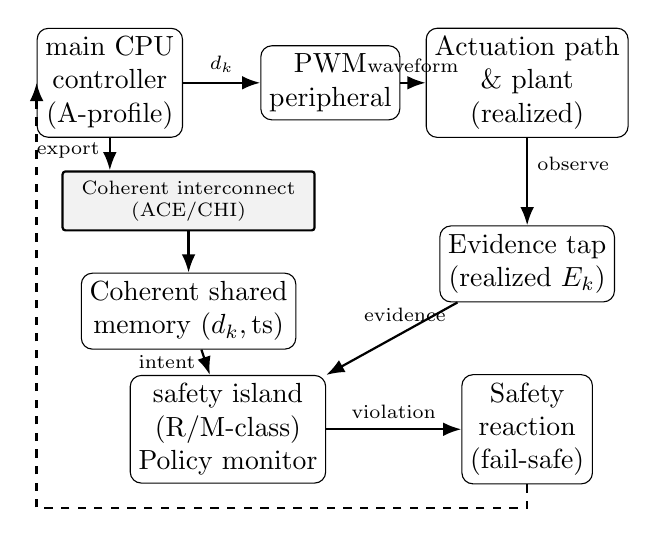
\begin{tikzpicture}[
      box/.style={draw,rounded corners,align=center,inner sep=3pt},
      arr/.style={-Latex,thick},
      lbl/.style={font=\scriptsize},
    ]
    %% === Row 1: Actuation chain ===
    \node[box] (ctrl) at (0,0)
      {\PrimaryCompute\\controller\\(A-profile)};
    \node[box] (pwm)  at (2.8,0)
      {PWM\\peripheral};
    \node[box] (plant) at (5.3,0)
      {Actuation path\\\& plant\\(realized)};

    \draw[arr] (ctrl) -- node[above,lbl]{$d_k$} (pwm);
    \draw[arr] (pwm)  -- node[above,lbl]{waveform} (plant);

    %% === Row 2: Coherent interconnect (left, does not span evidence) ===
    \node[draw,thick,fill=black!5,rounded corners=1pt,
          minimum width=32mm,minimum height=5mm,
          font=\scriptsize,align=center]
      (bus) at (1.0,-1.5)
      {Coherent interconnect\\(ACE/CHI)};

    %% === Evidence tap (right side, clearly separated from bus) ===
    \node[box] (evidence) at (5.3,-2.3)
      {Evidence tap\\(realized $E_k$)};

    %% === Shared memory (below bus) ===
    \node[box] (mailbox) at (1.0,-2.9)
      {Coherent shared\\memory ($d_k$,\,ts)};

    %% === Row 4: Safety island + reaction ===
    \node[box] (si) at (1.5,-4.4)
      {\SafetyIsland\\(R/M-class)\\Policy monitor};
    \node[box] (react) at (5.3,-4.4)
      {Safety\\reaction\\(fail-safe)};

    %% --- Intent-export path (left, through coherent fabric) ---
    \draw[arr] (ctrl.south) --
      node[left,lbl,pos=0.4]{\scriptsize export}
      (ctrl.south |- bus.north);
    \draw[arr] (bus) -- (mailbox);
    \draw[arr] (mailbox) --
      node[left,lbl]{intent} (si);

    %% --- Evidence path (right, independent observation) ---
    \draw[arr] (plant) --
      node[right,lbl,pos=0.3]{observe} (evidence);
    \draw[arr] (evidence) --
      node[above,lbl,pos=0.4]{evidence} (si);

    %% --- Reaction path ---
    \draw[arr] (si) --
      node[above,lbl]{violation} (react);
    \draw[arr,dashed] (react.south) -- ++(0,-0.3) -| (ctrl.west);
  \end{tikzpicture}
  \caption{Policy-level monitoring on a \SafetyIsland. The monitor reads controller intent exported via cache-coherent shared memory (left path) and independently acquires evidence of realized actuation (right path) to evaluate temporal safety policies online. On violation, the island triggers a safety reaction within the \FTTI.}
  \label{fig:arch}
\end{figure}

\subsection{Research Questions and Hypotheses}
We treat the \SafetyIsland monitor as an architecture design space and focus the project on answering the following questions:
\begin{itemize}
\item \textbf{RQ1 (Coherent interface).} How should the \SafetyIsland participate in cache-coherent sharing with the \PrimaryCompute (e.g., full coherent agent vs.\ coherent I/O), and what memory region and access controls minimize coupling while meeting latency?
\item \textbf{RQ2 (Snapshot and ordering).} What should the controller export (values plus timestamp/sequence information), and what synchronization rules over coherent shared memory ensure the \SafetyIsland reads consistent controller records (not mixed old/new fields)~\cite{Pulte2018SimplifyingARM,CleavelandTrippel2024MemGlue,Goens2023CompoundConsistency}?
\item \textbf{RQ3 (Predictability).} Under contention and coherence traffic, what worst-case intent-export and monitor latencies are achievable, and what coherence/policy mechanisms keep detection within the \FTTI~\cite{Hassan2017PredictableCoherence,Hassan2022IntegratingCOTSCoherence,Chisholm2016TensionIsolationSharing}?
\item \textbf{RQ4 (Evidence, time alignment, and monitor budget).} Where should we collect evidence of realized actuation (controller boundary vs.\ actuation boundary vs.\ plant-side signatures), how should evidence be time-stamped/aligned with controller records, and what class of temporal policies (e.g., \STL) and sampling rates are feasible on microcontroller-class safety islands within the \FTTI?
\end{itemize}

Our working hypothesis is that cache-coherent shared memory is the right substrate for low-latency intent export, and that with a small, explicit synchronization and predictability contract, a microcontroller-class \SafetyIsland can perform robust temporal-policy monitoring (e.g., \STL) within the \FTTI.

\subsection{Policy Language and Monitor Model}
We use \STL as a representative policy language for timing requirements over sampled signals, focusing on bounded time windows to support predictable runtime cost. Other temporal formalisms for sampled/metric signals could also be used; our architecture questions are about how policy monitors consume consistent and well-timed traces. For a signal $s(t)$, typical predicates are inequalities (e.g., $s(t)\leq \theta$) and relational checks between intended and realized actuation.

We adopt robust semantics where a monitor computes a robustness value $\rho(\varphi, t)$ such that $\rho<0$ implies violation and $|\rho|$ quantifies margin~\cite{FainekosPappas2009,Deshmukh2017}. Robustness is also a natural fit for CPS monitoring under bounded sensor noise and bounded time-alignment error between controller reports and evidence.

% \section{Soundness Argument (Sketch)}
% The proposal's soundness claim is conditional: it establishes that, under stated interface and timing assumptions, the \SafetyIsland's monitor decision corresponds to the semantics of the specified policy.

% \textbf{(1) Monitor correctness for robust \STL.} Given aligned traces for intended and realized signals, the monitor computes a robustness value $\rho(\varphi,t)$. When $\rho(\varphi,t)<0$, the property $\varphi$ is violated at time $t$ under robust semantics~\cite{Deshmukh2017}.

% \textbf{(2) Consistent controller snapshots.} If the controller record is exported via coherent shared memory using a synchronization discipline that prevents mixed old/new fields, then the \SafetyIsland evaluates policies over the intended command for that step. A key deliverable is to specify the minimal ordering rules (under the relevant memory models) that make this snapshot property true for an A-profile CPU paired with microcontroller-class cores~\cite{Pulte2018SimplifyingARM,CleavelandTrippel2024MemGlue,Goens2023CompoundConsistency}.

% \textbf{(3) Temporal alignment soundness.} If the evidence acquisition path guarantees that evidence $E_k$ corresponds to the same physical actuation interval as the controller record $d_k$ (within bounded skew), then the monitor evaluates predicates over the correct windows. Where skew is non-zero but bounded, we incorporate it into policy timing bounds and robustness thresholds.

% \textbf{(4) End-to-end reaction within \FTTI.} If the worst-case time to obtain a consistent controller record via coherent sharing, plus the monitor's worst-case execution time, plus actuation of the reaction is bounded by $\Delta \leq \FTTI$, then a detected violation can be controlled before it becomes a hazard (as required by functional safety practice)~\cite{ISO26262,NVIDIADriveFSI,Hassan2022IntegratingCOTSCoherence}.

\section{Case Study: PWM Actuation Integrity Policies}
PWM is a useful case study because it is ubiquitous in automotive actuation (traction inverter control, electric power steering, DC--DC conversion), and because PWM parameters provide a compact controller report while the realized waveform provides rich, independently measurable evidence.

In this case study, $d_{\text{int}}$ denotes the intended duty cycle from the exported controller record ($d_k$), and $d_{\text{real}}$ denotes a realized duty estimate derived from evidence $E_k$.

We will specify a small policy set that illustrates different monitoring needs:
\begin{itemize}
\item \textbf{Tracking integrity.} After each controller update, the realized duty cycle must converge to the intended value within a bound and remain within tolerance for a minimum dwell time:
$
\mathbf{G}\big(\mathrm{update} \rightarrow \mathbf{F}_{[0,\delta]} \mathbf{G}_{[0,\tau]}\big(|d_{\text{real}}-d_{\text{int}}|\le \epsilon\big)\big).
$
\item \textbf{Safety envelope.} When a safety condition is asserted (e.g., brake override, thermal derate), realized PWM must enter and stay within a conservative safe envelope within a deadline.
\item \textbf{Glitch exclusion.} Realized PWM must not contain pulses shorter than a minimum duration, capturing short-pulse glitches and related timing faults.
\end{itemize}
These examples emphasize that the monitor checks both the \emph{temporal} structure (deadlines, dwell) and the \emph{relation} between intended and realized actuation.

\section{Expected Contributions}
This project aims to contribute:
\begin{itemize}
\item A cache-coherent \SafetyIsland architecture for online \STL policy monitoring of CPS actuation paths, grounded in established safety-island practice and coherent interface standards~\cite{ArmAutoSolutionsOverview,NVIDIADriveFSI,ArmAMBA4,ArmAMBA5}.
\item A monitoring-oriented shared-memory contract: what the controller exports, what evidence is observed, and what ordering/predictability assumptions are required so the \SafetyIsland reads consistent snapshots and meets the \FTTI~\cite{Pulte2018SimplifyingARM,Hassan2017PredictableCoherence,Goens2023CompoundConsistency}.
\item A PWM actuation integrity case study (policies plus evidence choices) that makes the architectural questions concrete.
\end{itemize}

\section{Conclusion}
Runtime verification and functional safety supervision are often discussed separately: the former emphasizes specifications and monitoring, while the latter emphasizes trusted supervisory compute and bounded reaction times. This proposal connects them by putting a cache-coherent \SafetyIsland interface at the center: what the controller exports into shared memory, what evidence the island observes, and what ordering and predictability guarantees are needed for correct \STL policy checking under tight latency.

{\footnotesize
\bibliographystyle{plain}
\bibliography{references}
}

\end{document}
